%--------------------
% Packages
% -------------------
\documentclass[11pt,a4paper]{article}
\usepackage[utf8x]{inputenc}
\usepackage[T1]{fontenc}
%\usepackage{gentium}
\usepackage{mathptmx} % Use Times Font
\usepackage[table]{xcolor}
\usepackage{caption}
\usepackage{booktabs,makecell}

\usepackage[pdftex]{graphicx} % Required for including pictures
\usepackage[pdftex,linkcolor=black,pdfborder={0 0 0}]{hyperref} % Format links for pdf
\usepackage{calc} % To reset the counter in the document after title page
\usepackage{enumitem} % Includes lists
\usepackage[english]{babel}
\usepackage{natbib}
  \bibliographystyle{abbrvnat}
  \setcitestyle{authoryear}

\frenchspacing % No double spacing between sentences
\linespread{1.2} % Set linespace
\usepackage[a4paper, lmargin=0.1666\paperwidth, rmargin=0.1666\paperwidth, tmargin=0.1111\paperheight, bmargin=0.1111\paperheight]{geometry} %margins
%\usepackage{parskip}

\usepackage[all]{nowidow} % Tries to remove widows
\usepackage[protrusion=true,expansion=true]{microtype} % Improves typography, load after fontpackage is selected


%-----------------------
% Set pdf information and add title, fill in the fields
%-----------------------
\hypersetup{ 	
pdfsubject = {},
pdftitle = {GroupProjectDigitalToolsFinance},
pdfauthor = {}
}

%-----------------------
% Begin document
%-----------------------

\title{\textbf{Impact of Corona on the Swiss Market Index(SMI): \\ 
Which Branches were the Winners and Losers of the Crisis?}}
\author{Jirong Liu, Sandra Kuchenbecker, Meichen Shen, Wenxi Feng, Silin Zhou}
\date{14.12.2020}

\begin{document}

\maketitle
\centerline{Seminar: Digital Tools for Finance}
\centerline{Fall 2020}
\centerline{University of Zurich}
\tableofcontents
\newpage
\section{Introduction to the SMI}
Some general information about the SMI will be provided first, before the economic consequences of the corona crisis are stated in the following chapters. \\

\noindent The SMI was launched on 01.06.1988. It`s starting value was set at 1500 points. Since then it has established itself as a leading Swiss index for large companies.\\
The SMI is a blue-chip index. This means that it tracks shares of well-known, financially stable, publicly traded companies, so called \emph{blue-chips}. The investors can expect consistent returns, which make them desirable investment opportunities (\cite{JamesChen2019}).\\

\noindent The SMI includes the 20 largest stocks from the SPI, the Swiss performance index. Furthermore, the SMI covers about 80\% of the total capitalization of the Swiss stock market.\\
The index is free-float-adjusted. When calculating the market capitalization of the index's underlying companies, one takes the equity's price and multiplies it by the number of shares available in the market. The big contrast to the full-market indexes is that the latter calculates with both the active and inactive shares, when determining market capitalization while the SMI excludes locked-in shares, such as shares held by insiders, promoters or governments(\cite{JamesChen(2020)}).

\noindent That no component exceeds a weight of 20\%  is ensured by the limitation of the title weights. The SMI is thus in line with the ESMA UCITS guidelines and can therefore be used as a reference index for the Swiss stock market in the European Union(\cite{SIXSwissExchangeAG}).
It is published as a price index and as a performance index under the name SMIC (SMI dividend adjusted)(\cite{SIXSwissExchangeAG})
\noindent Because the SMI represents the Swiss stock market, it can be used as an \emph{underlying} for various financial products such as options, futures, structured products and exchange-traded funds(\cite{SIXSwissExchangeAG})

\noindent Like most other equity barometers, the Swiss benchmark index is shaped by macroeconomic and global economic events. The structure of the index allow that a maximum of 30 companies may be included in the barometer. In practice the number of members fluctuates between 18 and 29 companies (\cite{MichaelRasch}). The pie chart below shows the percentages which the industries occupy of the whole SMI index. Health care occupies the biggest percentage of the whole SMI. \\

\noindent The tables show the exact firms of all the industries. For each firm the market capitalisation is listed in Million Swiss Francs. The pie chart is from 2017 yet it becomes clear that even in data from December 2020 the constitution is similar.
\\
There are three tables. The first presents the two industry branches with the biggest share, followed by the two branches with medium shares and last but not least the two branches with the least shares of the whole SMI index.\\
\pagebreak
.
\newline

\newline
\begin{figure}[h]
    \centering
    \caption{Industry Weights as \% of the SMI(\cite{SIXSwissExchangeAG})}
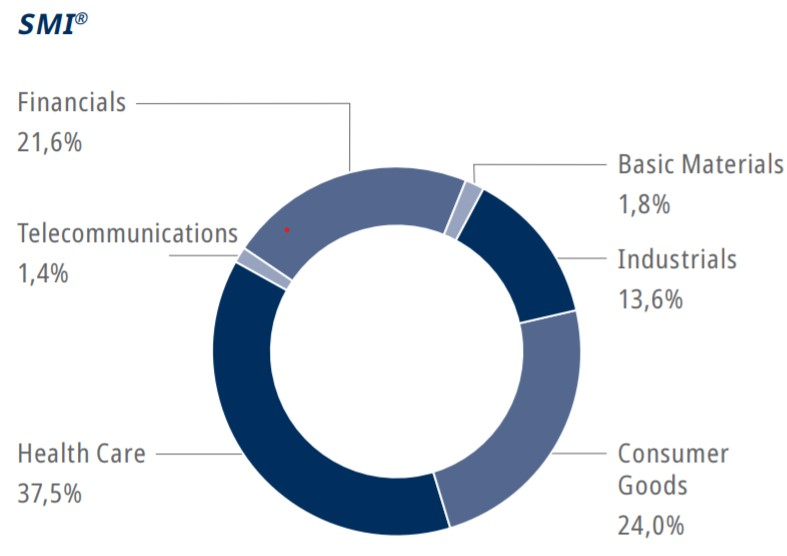
\includegraphics[width=90mm]{Pic.jpg}
\end{figure}

\\
.
\vspace{10mm}

\begin{table}[h]
\centering
\caption{Biggest SMI Branches - 2017(\cite{DieBoerse})}

\setlength{\arrayrulewidth}{0.5mm}
\setlength{\tabcolsep}{5pt}
\renewcommand{\arraystretch}{2}

{\rowcolors{4}{green!80!yellow!50}{green!70!yellow!40}
\begin{tabular}[c]{ |p{3cm}|p{3cm}|p{3cm}|p{3cm}|  }
\hline
\multicolumn{4}{|c|}{Index Composition and Marketcap.in Mio. CHF} \\
\hline
Branche & Mrkt. Cap. & Branche & Mrkt. Cap. \\
\hline
\textbf{HEALTH CARE} & \textbf{504'785.1} & \textbf{CONSUMER GOODS} & \textbf{328'564.2} \\
Roche & 257’909.69 & Nestlé & 275’286.32 \\
Novartis & 178’739.42 & Richemont & 41’699.01 \\
Lonza & 40’349.53 & Swatch Group & 11’578.86 \\
Alcon & 27’786.43 & - & - \\
\hline
\end{tabular}
}
\end{table}
\\ 
\pagebreak

\begin{table}[h]
\centering\caption{Medium SMI Branches - 2017(\cite{DieBoerse})}

\setlength{\arrayrulewidth}{0.5mm}
\setlength{\tabcolsep}{5pt}
\renewcommand{\arraystretch}{2}

{\rowcolors{4}{green!80!yellow!50}{green!70!yellow!40}
\begin{tabular}[c]{ |p{3cm}|p{3cm}| p{3cm}|p{3cm}| }
\hline
\multicolumn{4}{|c|}{Index Composition and Marketcap. in Mio. CHF} \\
\hline
Branche & Mrkt. Value & Branche & Mrkt. Value\\
\hline
\textbf{FINANCIALS} & \textbf{190'720.7}&\textbf{INDUSTRIALS} & \textbf{149'449.5} \\
UBS Group & 46’140.11 & ABB & 50’208.50 \\
Zurich Insurance & 54’118.04 & LafarageHolcim & 29’766.31 \\
CS Group & 28’568.49 & Sika & 31’586.44 \\
Partners Group & 25’556.94 & Geberit & 18’742.87 \\
Swiss RE & 23’321.46 & SGS SA & 19’145.34 \\
Swiss life Holding & 13’015.70 & - & - \\
\hline
\end{tabular}
}
\end{table}

\begin{table}[h]
\centering
\caption{Smallest SMI Branches - 2017(\cite{DieBoerse})}
\setlength{\arrayrulewidth}{0.5mm}
\setlength{\tabcolsep}{5pt}
\renewcommand{\arraystretch}{2}
{\rowcolors{4}{green!80!yellow!50}{green!70!yellow!40}
\begin{tabular}[c]{ |p{3cm}|p{3cm}|p{3cm}|p{3cm}| }
\hline
\multicolumn{4}{|c|}{Index Composition and Marketcap. in Mio} \\
\hline
Branche & Mrkt. value & Branche & Mrkt. Value\\
\hline
\textbf{MATERIALS} & \textbf{32’628.50} &\textbf{TELECOMMUN.} & \textbf{24’593.06} \\
Givaudan & 32’628.50 & Swisscom & 24’593.06 \\
\hline
\end{tabular}
}
\end{table}
\\ 
\noindent Over the past 3 years only 2 position occupations have changed. Now that the index has been presented ,the following chapters will show the effects of the corona crisis 2020 on the Swiss economy.\\ 
\newpage

\section{Economic Consequences due to Corona Crisis}

Compared to other countries globally, Switzerland was not as rattled by the crisis. The first infection was determined in Ticino in February 2020(\cite{BundesamtFürGesundheit}). 
On December 7th 2020 Switzerland had 354 306 cases of corona, over 5000 people had died of the virus(\cite{Worldometer(2020)}).
Swiss politicians are still struggling to find the ideal way to conquer the meanwhile second outbreak, while at the same time trying to appease the Swiss population which is in fear of a radical lockdown during the Christmas holidays if the number of infections continues to rise. There is hope for the future in that vaccines are being produced and the enhancement of restrictions could hopefully result in a reduced infection rate by next spring. However, when analysing the crisis from a purely economic perspective, the Swiss economy has definitely suffered from the trade slumps. Generally, the crisis has not spared any branch. Some consequences are more obvious than others. The summer tourism as well as the approaching ski and winter tourism will be severely limited. This has consequences for the Swiss economy as well. \\
Due to the lockdown many employers had establish home-office or short-time work. The state has tried to support the economy with monetary aid packages. After the Gross Domestic Product (GDP) collapsed by 9\% during the first half of the year (\cite{HandelszeitungUndBilanz})the state approved of an aid package worth 65billion Swiss francs (\cite{PaulineTuruban(2020)}). However the export or import trade cannot be helped with such simple measures.The export trade has collapsed by almost 4\% and services by almost 15\% due to the lack of tourism, transport and cross-border interactions, as mentioned above (\cite{HandelszeitungUndBilanz}).

\\
\section{Specific Influence of Corona Crisis on the SMI}

\\
It can be stated with certainty that COVID-19 had a negative impact on Swiss stock market returns.
The key question now is how the corona crisis affected the SMI. The developments can be seen in the following plot. It shows the development of the SMI Index from February to December 2020. The slumps clearly show the shocks induced by the corona waves (\cite{DOminicBenz}).\\
Generally the whole Swiss economy suffered from the crisis. We can compare the firms of the SMI and their share price performance 

\vspace{20mm}

\newline
\begin{figure}[h]
    \centering
    \caption{Development of SMI 2020 - Corona Waves and Effect on Economy(\cite{Investopedia(2020)}}
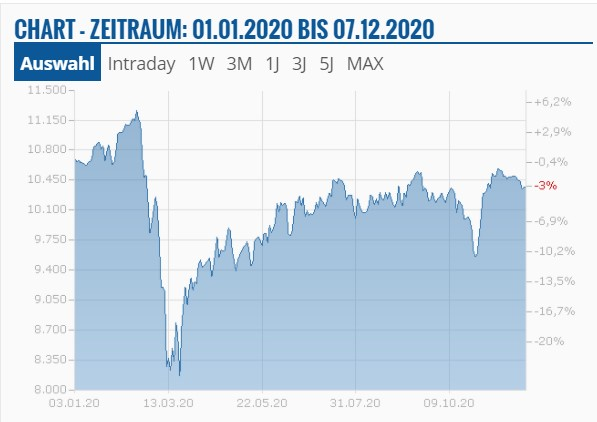
\includegraphics[width=130mm]{AktuellSMI.jpg}
\end{figure}

\\
\newpage
The two corona waves can clearly be seen in the development of the index.The second wave did not have such a grave impact in comparison to the first wave. The share prices did not drop as severely as they did in the beginning of the year. The general trend shows that the biggest losses were recorded primarily by so-called cyclical stocks.In general the SMI dropped by ~ 3\% in the last quarter.\\
The prices were primarily burdened by worries about the Chinese economy as various data indicated a weakening of growth. As a result, the stock exchange plummeted.In addition to this, the devaluation of the Chinese currency yuan by the central bank in August additionally burdened the financial sector. The other worrying factor was the insecurity concerning the interest rate reversal in the USA. In September the US-Note bank Chief Janet Yellen had postponed her Zero-interest politics, based on the global insecurities (\cite{DOminicBenz}). 
The significant winner of the crisis is Nestle. Nestle actually managed to gain 8,5\% during July and September. This is surprising as Nestle is one of the most criticised companies in Switzerland, due to their immoral capitalization of water and exploitation of third world countries (\cite{JanaGlose}). The second company which did not loose during the corona crisis was the Swiss RE.The insurance-re-insurer could profit as, apart from corona, they were spared from the usual profit reducing natural disasters.\\
Richemont and Swatch also had less losses than expected. The shares of Richemont only reduced by 1,9\% and Swatche`s by 3\%, which is minimal in comparison to the other companies. 
Share owners of the Credit Suisse however lost around 9\%. The UBS shares also lost. 
\\
\\
The biggest loser in this aspect however were share owners of Transocean. The share owners of Syngenta also had to cope with huge course loses in comparison to the other firms listed on the SMI.Another huge loser of the corona crisis was LafargeHolfim, which lost almost a third of its worth by October, as the shares are very dependent on cycles (\citet{DOminicBenz}). 
\\
In summary the corona crisis had significant influences on all parts of the Swiss society. The health system was over burdened and the usual human interactions and working together had to be restructured.Most importantly the Swiss politicians and public figures are still trying to find ways to steer the economy out of the crisis. It is a positive sign to see the index recover and that the second wave did not lead to such a massive shock as the first corona wave did. 
\\
\newpage

\bibliography{references.bib}
\end{document}
